% !TeX root = ../../main.tex
\documentclass[../AAE590LGM_HW3.tex]{subfiles}
\begin{document}

\subsection{4.a) and 4.b) \textbf{Dynamics as Mixed Invariant on $\SEt{2}$ and Adding Wind (World-Frame):}}
\underline{Question}: \\
Test group affine property for fixed wing aircraft dynamics with and without wind \\
\underline{Solution}: \\
Code snippet 5 shows the verification of group affine property of the $\SEt{2}$ windy fixed wing aircraft dynamics
\lstinputlisting[language=Python,caption={$\SEt{2}$ Fixed Wing Aircraft Group Affine Test}, inputpath=../../../Tests/SE22]{test_SE22_group_affine.py}

\begin{figure}[H]
    \caption{Windless and Windy Fixed Wing Aircraft Group Affine Test Passing}
    \centering
    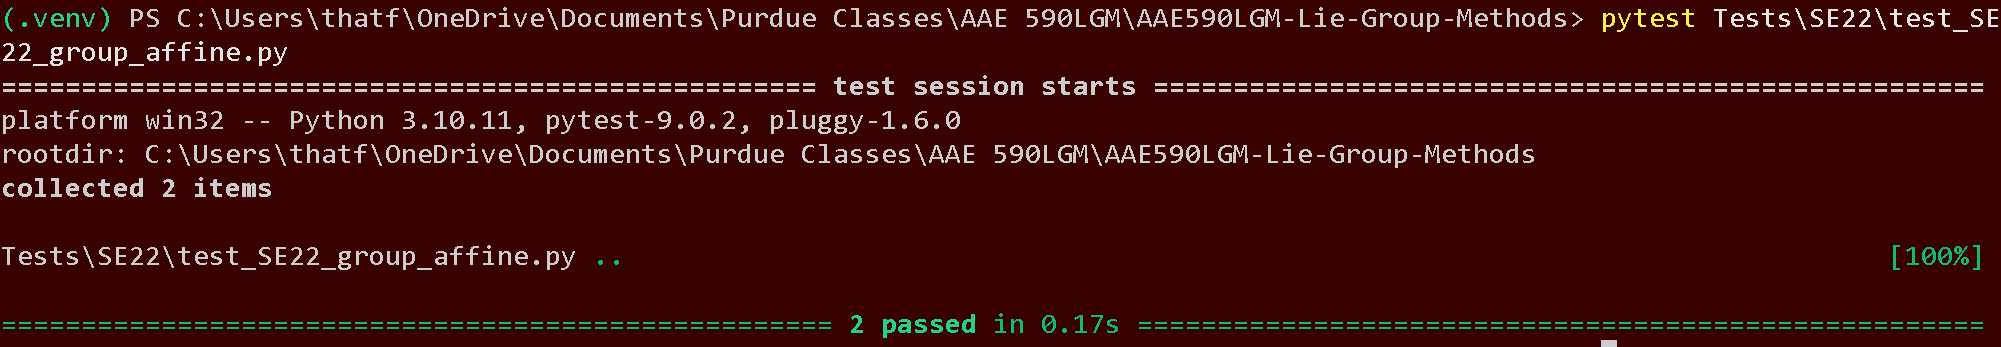
\includegraphics[width=0.7\linewidth]{AAE590LGM_HW3_Q4_gfckpass.png}
\end{figure}

\subsection{4.c) 2D INS Simulator}
\lstinputlisting[language=Python,caption={2D INS Simulator Code}]{AAE590LGM_HW3_Q4.py}


\begin{figure}[H]
    \caption{Plots of trajectory}
    \centering
    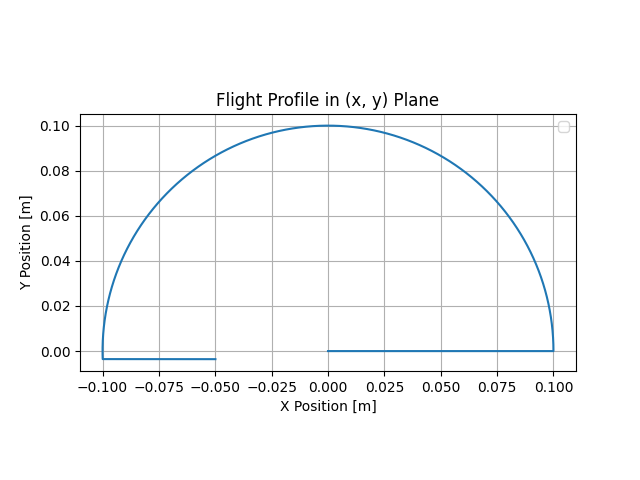
\includegraphics[width=0.7\linewidth]{AAE590LGM_HW3_Q4_traj.png}
\end{figure}

\begin{figure}[H]
    \caption{Plots of velocity}
    \centering
    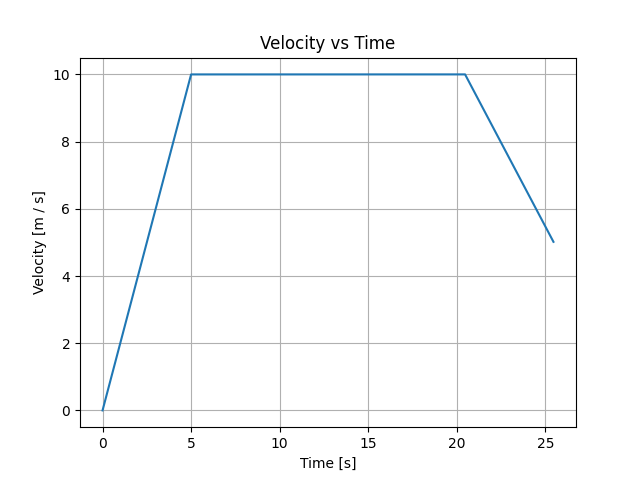
\includegraphics[width=0.7\linewidth]{AAE590LGM_HW3_Q4_vel.png}
\end{figure}

\begin{figure}[H]
    \caption{Plots of heading}
    \centering
    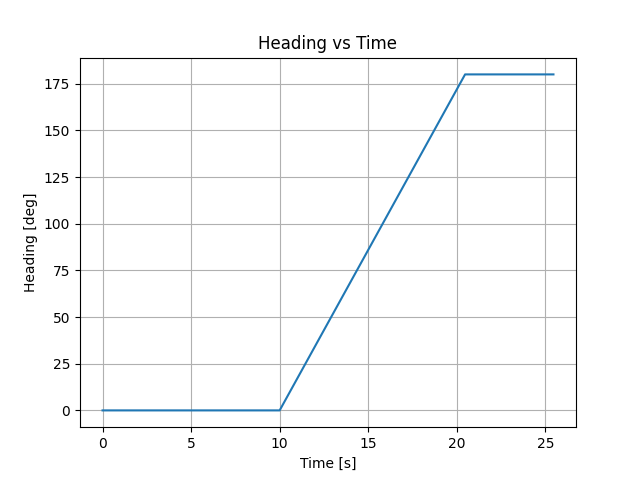
\includegraphics[width=0.7\linewidth]{AAE590LGM_HW3_Q4_head.png}
\end{figure}

Spiral test
\begin{figure}[H]
    \caption{Plots of Spiral}
    \centering
    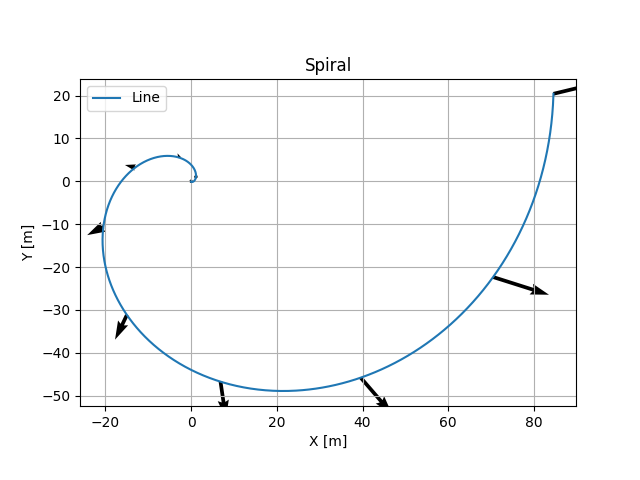
\includegraphics[width=0.7\linewidth]{AAE590LGM_HW3_Q4_spiral.png}
\end{figure}

\begin{figure}[H]
    \caption{Plots of Spiral velocity}
    \centering
    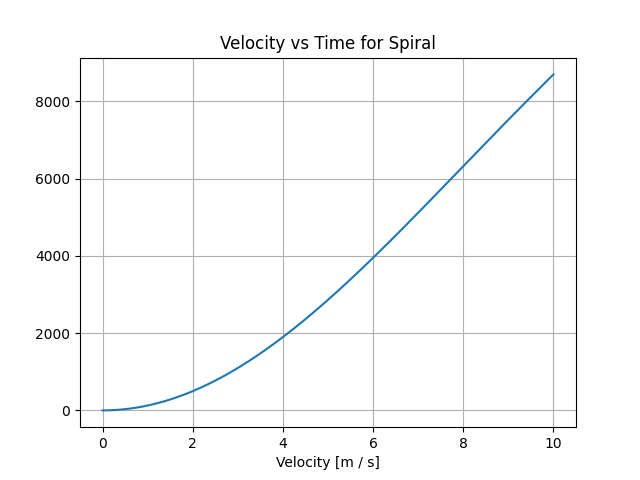
\includegraphics[width=0.7\linewidth]{AAE590LGM_HW3_Q4_spiralvel.png}
\end{figure}

\end{document}